%%%%%%%%%%%%%%%%%%%%%%%%%%%%%%%%%%%%%%%%%
% Maggi Memoir Thesis
% XeLaTeX Template
% Version 1.0 (22/12/13)
%
% This template has been downloaded from:
% http://www.LaTeXTemplates.com
%
% Original authors:
% Federico Maggi (fede@maggi.cc) with extensive modifications by:
% Vel (vel@latextemplates.com)
%
% License:
% CC BY-NC-SA 3.0 (http://creativecommons.org/licenses/by-nc-sa/3.0/)
%
% Important notes:
% This template needs to be compiled with XeLaTeX.
%
% Most of the document content and packages are specified within structure.tex
% so if you need to make modifications to the template have a look there first!
%
% This template uses several fonts that are not available on most operating 
% systems by default. These are: Adobe Caslon Pro, Envy Code R and 
% Optima Regular. You will either need to obtain these and install them on your
% system or change them to different fonts. Simply go to the Fonts block just
% below here and modify their names to other fonts. You can also comment them 
% out completely to use the default LaTeX font.
%
%%%%%%%%%%%%%%%%%%%%%%%%%%%%%%%%%%%%%%%%%

%----------------------------------------------------------------------------------------
%	PACKAGES AND OTHER DOCUMENT CONFIGURATIONS
%----------------------------------------------------------------------------------------

\documentclass[10pt,showtrims,a4paper,twoside]{memoir} % Change font size here (allowable values are 9pt-12pt), change the paper size, specify one or two sided printing and specify whether to show trimming lines

%----------------------------------------------------------------------------------------
%	VARIOUS REQUIRED PACKAGES AND CONFIGURATIONS
%----------------------------------------------------------------------------------------

\XeTeXinputencoding latin1
\usepackage[T1]{fontenc} % Support for more character glyphs
\usepackage[round]{natbib}\citeindextrue % Round brackets around citations, change to square for square brackets
\usepackage{graphicx} % Required to include images
\usepackage{color} % Required for custom colors
\usepackage{amsmath,amssymb,theorem} % Math packages
\usepackage{listings} % Required for including snippets of code
\usepackage{booktabs} % Required for better horizontal rules in tables
\usepackage{xspace} % Provides the ability to use an intelligent space which is used in \institution and \department
\usepackage[printonlyused,withpage]{acronym} % Include a list of acronyms
\usepackage{rotating} % Allows tables and figures to be rotated
\usepackage{hyperref} % Required for links and changing link options
\usepackage{fontspec} % Required for specifying custom fonts in XeTeX
\usepackage{microtype} % Slightly tweak font spacing for aesthetics

\hypersetup{colorlinks, breaklinks, linkcolor=black,citecolor=black,filecolor=black,urlcolor=black} % Set up hyperlinks including colors for references, urls and citations

%\definecolor{c64}{rgb}{.063,0,.612} % Example color definition, the color can be used with the \color{name} command

\makeatletter
\renewcommand{\fnum@figure}{\textsc{\figurename~\thefigure}} % Make the "Figure 1.1" text in small caps
\makeatother

%----------------------------------------------------------------------------------------
%	PAGE LAYOUT
%----------------------------------------------------------------------------------------

% The memoir class used in this template contains the ability to set the stock paper size and the trimmed size independently. It also has the ability to show trim lines showing where stock paper should be trimmed to get the final book size. This can all be a bit confusing so please see the memoir class documentation for more information.

% By default, the paper size is a4paper which is 29.7cm × 21cm. To change this, simply change "a4paper" in the \documentclass[a4paper,...]{memoir} command in thesis.tex to another size such as "letterpaper".
% By default, the trimmed size is 24cm x 17cm and trim lines are shown. To remove trim lines, simply remove "showtrims" from the \documentclass[showtrims,...]{memoir} command in thesis.tex. The size of the trimmed content is set with the \settrimmedsize{}{} command below.
% If you wish to remove trims and set the content to fit the paper size (i.e. no trimming at all), all you have to do is remove "showtrims" as above and comment out the \settrimmedsize{}{} command below.

%\setstocksize{24cm}{17cm} % Uncomment to manually set the stock size and override the setting in \documentclass
\settrimmedsize{24cm}{17cm}{*} % Change the trimmed area size or comment out this line entirely to fit the content to the paper size without trimming
\setlrmarginsandblock{37.125mm}{*}{0.9} % The first bracket specifies the spine margin, the second the edge margin and the third the ratio of the spine to the edge. Only one or two values are required and the remaining one(s) can be a star (*) to specify it is not needed. By default the edge margin is 10% smaller and 
\setulmarginsandblock{37.125mm}{*}{*} % The first bracket specifies the upper margin, the second the lower margin and the third the ratio of the upper to the lower. Only one or two values are required and the remaining one(s) can be a star (*) to specify it is not needed.
\setmarginnotes{17pt}{51pt}{\onelineskip} % The size of marginal notes, the three values in curly brackets are \marginparsep, \marginparwidth and \marginparpush
\setheadfoot{\onelineskip}{2\onelineskip} % Sets the space available for the header and footer
\setheaderspaces{*}{2\onelineskip}{*} % Sets the spacing above and below the header
\setlength{\trimtop}{0pt} % Sets the spacing above the trimmed area, i.e. moved the trimmed area down the page if positive

% Comment the two lines below to reverse the position of the trimmed content on the stock paper, i.e. odd pages will have content on the right side instead of the left and even pages will have content on the left side instead of the right
\setlength{\trimedge}{\stockwidth}
\addtolength{\trimedge}{-\paperwidth}

\checkandfixthelayout % Makes sure your specifications are correct and implements them in the document

%----------------------------------------------------------------------------------------
%	CHAPTER HEADING STYLE
%----------------------------------------------------------------------------------------

\makeatletter
\makechapterstyle{thesis}{
\renewcommand{\chapternamenum}{}
\setlength{\beforechapskip}{0pt}
\setlength{\midchapskip}{0pt}
\setlength{\afterchapskip}{0pt}
\renewcommand{\chapnamefont}{\LARGE}
\renewcommand{\chapnumfont}{\chapnamefont}
\renewcommand{\chaptitlefont}{\chapnamefont}
\renewcommand{\printchapternum}{}
\renewcommand{\afterchapternum}{}
\renewcommand{\printchaptername}{}
\renewcommand{\afterchaptertitle}{\chapnumfont\hfill\thechapter\\\vspace*{-.3cm}\hrulefill\vspace*{6cm}\\}
}
\makeatother

%----------------------------------------------------------------------------------------
%	TABLE OF CONTENTS DEPTH
%----------------------------------------------------------------------------------------

\maxsecnumdepth{subsubsection}
\maxtocdepth{subsection}

%----------------------------------------------------------------------------------------
%	MATH THEOREM DEFINITIONS
%----------------------------------------------------------------------------------------

\theoremstyle{plain}
\newtheorem{thm}{Theorem}[section] % Defines the theorem environment
\newtheorem{prop}[thm]{Proposition} % Defines the proposition environment
\newtheorem{proof}{Proof}[section] % Defines the proof environment
\newtheorem{definition}{Definition}[section] % Defines the definition environment
\newtheorem{example}{Example}[section] % Defines the example environment
\newtheorem{rem}{Remark} % Defines the remark environment
\newtheorem{note}{Note}[section] % Defines the note environment

%----------------------------------------------------------------------------------------
%	CODE SNIPPET CONFIGURATION
%----------------------------------------------------------------------------------------

\lstset{
  basicstyle=\ttfamily\small,
  basewidth=0.55em,
  showstringspaces=false,
  numbers=left,
  numberstyle=\tiny,
  numbersep=2.5pt,
  keywordstyle=\bfseries\ttfamily,
  breaklines=true
}
% Examples of list environments for different programming languages, you will likely need to specify your own
\lstnewenvironment{pseudoc}{\lstset{frame=lines,language=C,mathescape=true}}{}
\lstnewenvironment{logs}{\lstset{frame=lines,basicstyle=\footnotesize\ttfamily,numbers=none}}{}
\lstnewenvironment{cc}{\lstset{frame=lines,language=C}}{}
\lstnewenvironment{c64}{\lstset{backgroundcolor=\color{c64},basewidth=0.65em,basicstyle=\commodoreface\color{c64light},numbers=none,framerule=10pt,rulecolor=\color{c64light},frame=tb,framexbottommargin=30pt}}{}
\lstnewenvironment{html}{\lstset{frame=lines,language=html,numbers=none}}{}
\lstnewenvironment{pseudo}{\lstset{frame=lines,mathescape=true,morekeywords={learn_string_domain, save_model}}}{}
\lstnewenvironment{pseudoctiny}{\lstset{language=C,mathescape=true,basicstyle=\tiny\sffamily}}{}
\lstnewenvironment{cctiny}{\lstset{language=C,basicstyle=\tiny\sffamily}}{}
\lstnewenvironment{pseudotiny}{\lstset{mathescape=true,basicstyle=\tiny\sffamily}}{} % Include the file containing the code defining the structure and style of the document

%------------------------------------------------
% Thesis Information

\title{Integrated Detection of Anomalous Behavior of Computer Infrastructures} % Thesis title

\author{Federico Maggi} % Author name

\date{December 2013} % The date

\newcommand{\institution}{University of California\xspace} % University/institution name

\newcommand{\department}{Department of Computer Science\xspace} % Department name

%------------------------------------------------
% Fonts

\defaultfontfeatures{Mapping=tex-text}
\setromanfont[Ligatures={Common}]{Adobe Caslon Pro} % Normal document font
\setmonofont[Scale=0.8]{Envy Code R} % Mono spaced font (\texttt{})
\setsansfont[Scale=0.9]{Optima Regular} % Sans-serif font (\textsf{})

\renewcommand*{\acffont}[1]{{\normalsize\itshape #1}} % Font style for the acronym text (e.g. Do It Yourself)
\renewcommand*{\acfsfont}[1]{{\normalsize\upshape #1}} % Font style for the acronym in bracket (e.g. (DIY))

%------------------------------------------------
% Hyphenations

\hyphenation{a-no-ma-lous a-no-ma-ly amounts breaches} % Specify custom hyphenation points in words with dashes where you would like hyphenation to occur, or alternatively, don't put any dashes in a word to stop hyphenation altogether

%----------------------------------------------------------------------------------------
%	TITLE PAGE
%----------------------------------------------------------------------------------------

\renewcommand{\maketitlehooka}{
\centering

\includegraphics[width=2.5cm]{Figures/polimi-logo}\\[.5cm] % Institution logo
\institution\\ % Print institution name
\emph{\department}\\[.2cm] % Print department name
DOTTORATO DI RICERCA IN INGEGNERIA DELL'INFORMAZIONE % Degree or other information
\par
\hrulefill
\vfill}
\renewcommand{\maketitlehookb}{\vfill}
\renewcommand{\maketitlehookc}{
\vfill
\begin{flushleft}
Advisor:\\
\textbf{Prof. Stefano Zanero}\\[.3cm] % Advisor's/supervisor's name
Tutor:\\
\textbf{Prof. Letizia Tanca}\\[.3cm] % Tutor's name
Supervisor of the Doctoral Program:\\
\textbf{Prof. Patrizio Colaneri} % Doctoral program supervisor's name
\end{flushleft}
\vfill}
\preauthor{\begin{flushright}Doctoral Dissertation of:\\\bfseries} % Text prior to the author name - right aligned and bold
\postauthor{\end{flushright}} % After the author name, stop right alignment

%----------------------------------------------------------------------------------------

\makeindex % Write an index file

\begin{document}

\begin{titlingpage}
\maketitle % Print the title page
\end{titlingpage}

\frontmatter % Use roman page numbering style (i, ii, iii, iv...) for the pre-content pages

%----------------------------------------------------------------------------------------
%	PREFACE
%----------------------------------------------------------------------------------------

\section*{Preface}
This thesis embraces all the efforts that I put during the last three years as a PhD student at Politecnico di Milano. I have been working under the supervision of Prof. S. Zanero and Prof. G. Serazzi, who is also the leader of the research group I am part of. In this time frame I had the wonderful opportunity of being ``initiated'' to research, which radically changed the way I look at things: I found my natural \emph{``thinking outside the box''} attitude --- that was probably well-hidden under a thick layer of lack-of-opportunities, I took part of very interesting joint works --- among which the year I spent at the Computer Security Laboratory at UC Santa Barbara is at the first place, and I discovered the Zen of my life.

My research is all about \emph{computers} and every other technology possibly related to them. Clearly, the way I look at computers has changed a bit since when I was seven. Still, I can remember me, typing on that \textsf{Commodore} 64 in front of a tube TV screen, trying to get that d---n routine written in \textsf{Basic} to work. I was just playing, obviously, but when I recently found a picture of me in front of that screen...it all became clear.

So, although my attempt of writing a program to authenticate myself was a little bit naive --- being limited to a print instruction up to that point apart, of course --- I thought \emph{``maybe I am not in the wrong place, and the fact that my research is still about security is a good sign''}!

Many years later, this work comes to life. There is a humongous amount of people that, directly or indirectly, have contributed to my research and, in particular, to this work. Since my first step into the lab, I will not, ever, be thankful enough to Stefano, who, despite my skepticism, convinced me to submit that application for the PhD program. For trusting me since the very first moment I am thankful to Prof. G. Serazzi as well, who has been always supportive. For hosting and supporting my research abroad I thank Prof. G. Vigna, Prof. C. Kruegel, and Prof. R. Kemmerer. Also, I wish to thank Prof. M. Matteucci for the great collaboration, Prof. I. Epifani for her insightful suggestions and Prof. H. Bos for the detailed review and the constructive comments.

On the colleagues-side of this acknowledgments I put all the fellows of Room 157, Guido, the crew of the seclab and, in particular, Wil with whom I shared all the pain of paper writing between Sept '08 and Jun '09.

On the friends-side of this list Lorenzo and Simona go first, for being our family.

I have tried to translate in simple words the infinite gratitude I have and will always have to Valentina and my parents for being my fixed point in my life. Obviously, I failed.

\begin{flushright}
\textsc{\theauthor}\\
Milano\\
September 2009
\end{flushright}

\cleartoverso % Force a break to an even page

%----------------------------------------------------------------------------------------
%	ABSTRACT
%----------------------------------------------------------------------------------------

\begin{abstract}
This dissertation details our research on anomaly detection techniques, that are central to several classic security-related tasks such as network monitoring, but it also have broader applications such as program behavior characterization or malware\index{malware} classification. In particular, we worked on anomaly detection from three different perspective, with the common goal of recognizing awkward activity on computer infrastructures. In fact, a computer system has several weak spots that must be protected to avoid attackers to take advantage of them. We focused on protecting the operating system, central to any computer, to avoid malicious code to subvert its normal activity. Secondly, we concentrated on protecting the web applications, which can be considered the modern, shared operating systems; because of their immense popularity, they have indeed become the most targeted entry point to violate a system. Last, we experimented with novel techniques with the aim of identifying related events (e.g., alerts reported by intrusion detection systems) to build new and more compact knowledge to detect malicious activity on large-scale systems.

Our contributions regarding host-based protection systems focus on characterizing a process' behavior through the system calls invoked into the kernel. In particular, we engineered and carefully tested different versions of a multi-model detection system using both stochastic and deterministic models to capture the features of the system calls during normal operation of the operating system. Besides demonstrating the effectiveness of our approaches, we confirmed that the use of finite-state, deterministic models allow to detect deviations from the process' control flow with the highest accuracy; however, our contribution combine this effectiveness with advanced models for the system calls' arguments resulting in a significantly decreased number of false alarms.

Our contributions regarding web-based protection systems focus on advanced training procedures to enable learning systems to perform well even in presence of changes in the web application source code --- particularly frequent in the Web 2.0 era. We also addressed data scarcity issues that is a real problem when deploying an anomaly detector to protect a new, never-used-before application. Both these issues dramatically decrease the detection capabilities of an intrusion detection system but can be effectively mitigated by adopting the techniques we propose.

Last, we investigated the use of different stochastic and fuzzy models to perform automatic alert correlation, which is as post processing step to intrusion detection. We proposed a fuzzy model that formally defines the errors that inevitably occur if time-based alert aggregation (i.e., two alerts are considered correlated if they are close in time) is used. This model allow to account for measurements errors and avoid false correlations due to delays, for instance, or incorrect parameter settings. In addition, we defined a model to describe the alert generation as a stochastic process and experimented with non-parametric statistical tests to define robust, zero-configuration correlation systems.

The aforementioned tools have been tested over different datasets --- that are thoroughly documented in this document --- and lead to interesting results.
\end{abstract}

\cleartoverso % Force a break to an even page

%----------------------------------------------------------------------------------------
%	TABLE OF CONTENTS
%----------------------------------------------------------------------------------------

\tableofcontents* % Print the table of contents

\cleartoverso % Force a break to an even page

%----------------------------------------------------------------------------------------
%	LIST OF FIGURES
%----------------------------------------------------------------------------------------

\listoffigures % Print the list of figures

\cleartoverso % Force a break to an even page

%----------------------------------------------------------------------------------------
%	LIST OF TABLES
%----------------------------------------------------------------------------------------

\listoftables % Print the list of tables

\cleartoverso % Force a break to an even page

%----------------------------------------------------------------------------------------
%	ACRONYMS
%----------------------------------------------------------------------------------------

\chapter{List of Acronyms}
\begin{acronym}\addtolength{\itemsep}{-\baselineskip}
  \acro{AIC}{Akaike Information Criterion}
  \acro{ARMA}{Auto Regressive Moving Average}
  \acro{ARMAX}{Auto Regressive Moving Average eXogenous}
  \acro{ARX}{Auto Regressive eXogenous}
  \acro{AR}{Auto Regressive}
  \acro{ARR}{Alert Reduction Rate}
  \acro{ANSI}{American National Standard Institute}
  \acro{ASCII}{American Standard for Information Interxchange}
  \acro{BIC}{Bayesian Information Criterion}
  \acro{BMU}{Best Matching Unit}
  \acro{BSM}{Basic Security Module}
  \acro{CDF}{Cumulative Density Function}
  \acro{CDX}{Cyber Defense eXercise}
  \acro{CIA}{Confidentially Integrity Availability}
  \acro{CIDS}{Collaborative IDS}
  \acro{CPU}{Central Processing Unit}
  \acro{CSV}{Comma Separated Values}
  \acro{CTF}{Capture The Flag}
  \acro{DAG}{Direct Acyclic Graph}
  \acro{DARPA}{Defense Advanced Research Projects Agency}
  \acro{DB}{DataBase}
  \acro{DBMS}{DataBase Management System}
  \acro{DIDS}{Distributed IDS}
  \acro{DNS}{Domain Name System}
  \acro{DOM}{Document Object Model}
  \acro{DoS}{Denial of Service}
  \acro{DR}{Detection Rate}
  \acro{DTD}{Document Type Definition}
  \acro{ED}{Elementary Detector}
  \acro{ELF}{Executable Linux Format}
  \acro{FN}{False Negative}
  \acro{FNR}{False Negative Rate}
  \acro{FPR}{False Positive Rate}
  \acro{FP}{False Positive}
  \acro{FSA}{Finite State Automaton}
  \acro{FTP}{File Transfer Protocol}
  \acro{GCI}{Granger Causality Index}
  \acro{GCT}{Granger Causality Test}
  \acro{HIDS}{Host-based Intrusion Detection System}
  \acro{HMM}{Hidden Markov Model}
  \acro{HTML}{HyperText Markup Language}
  \acro{HTTP}{HyperText Transfer Protocol}
  \acro{ICD}{Idealized Character Distribution}
  \acro{IDEVAL}{Intrusion Detection eVALuation}
  \acro{IDMEF}{Intrusion Detection Message Exchange Format}
  \acro{IDS}{Intrusion Detection System}
  \acro{IDWG}{Intrusion Detection Working Group}
  \acro{ID}{Intrusion Detection}
  \acro{IETF}{Internet Engineering Task Force}
  \acro{IODEF}{Incident Object Description and Interchange Format}
  \acro{IPS}{Intrusion Protection System}
  \acro{ISP}{Internet Service Provider}
  \acro{IP}{Internet Protocol}
  \acro{IR}{Information Retrieval}
  \acro{IRC}{Internet Relay Chat}
  \acro{ISS}{Internet Security Systems}
  \acro{JSON}{JavaScript Object Notation}
  \acro{KBS}{Knowledge Base System}
  \acro{KS}{Kolmogorov-Smirnoff}
  \acro{LARIAT}{Lincoln Adaptable Real-time Information Assurance Testbed}
  \acro{LERAD}{Learning Rules for Anomaly Detection}
  \acro{LL}{Lincoln Laboratory}
  \acro{MDL}{Minimum Description Length}
  \acro{MIT}{Massachusetts Institute of Technology}
  \acro{ML}{Maximum Likelihood}
  \acro{MTU}{Maximum Transfer Unit}
  \acro{NIDES}{Next-generation Intrusion Detection Expert System}
  \acro{NIDS}{Network-based Intrusion Detection System}
  \acro{NNID}{Neural Network Intrusion Detection}
  \acro{NSTISSC}{National Security Telecomm. and Information Systems Sec. Committee}
  \acro{NTP}{Network Time Protocol}
  \acro{PC}{Program Counter}
  \acro{PDF}{Probability Density Function}
  \acro{PHAD}{Packet Header Anomaly Detection}
  \acro{PHP}{PHP Hypertext Preprocessor}
  \acro{PID}{Process IDentifier}
  \acro{ROC}{Receiving Operating Characteristic}
  \acro{SADE}{Syscall Sequence Arguments Anomaly Detection Engine}
  \acro{SDEE}{Security Device Event Exchange}
  \acro{SMTP}{Simple Message Transfer Protocol}
  \acro{SOM}{Self Organizing Map}
  \acro{SQL}{Structured Query Language}  
  \acro{SRI}{Stanford Research Institute}
  \acro{SSH}{Secure SHell}
  \acro{STATL}{State Transition Analysis Technique Language}
  \acro{SVN}{SubVersioN}
  \acro{SYN}{SYNchronize}
  \acro{TCP}{Trasmission Control Protocol}
  \acro{TF}{Truth File}
  \acro{TN}{True Negative}
  \acro{TNR}{True Negative Rate}
  \acro{TOS}{Type Of Service}
  \acro{TP}{True Positive}
  \acro{TTL}{Time To Live}
  \acro{UCSB}{University of California Santa Barbara}
  \acro{ULISSE}{Unsupervised Learning IDS with 2-Stages Engine}
  \acro{UDP}{User Datagram Protocol}
  \acro{UML}{Unified Modeling Language}
  \acro{URL}{Uniform Resource Locator}
  \acro{VPN}{Virtual Private Network}
  \acro{XML}{eXtensible Markup Language}
  \acro{XSD}{XML Schema Definition}
  \acro{XSS}{Cross-Site Scripting}
\end{acronym} % Include a List of Acronyms section using acronyms.tex where they are defined

\cleartoverso % Force a break to an even page

%----------------------------------------------------------------------------------------
%	COLOPHON
%----------------------------------------------------------------------------------------

\thispagestyle{empty} % Remove all headers and footers from this page

\vspace*{2em}
\renewcommand{\abstractname}{Colophon}
\begin{abstract}
This document was typeset using the \textsf{XeTeX} typesetting system created by the Non-Roman Script Initiative and the memoir class created by Peter Wilson. The body text is set 10pt with~Adobe Caslon Pro. Other fonts include \texttt{Envy Code R}, \textsf{Optima Regular} and. Most of the drawings are typeset using the \textsf{TikZ/PGF} packages by Till Tantau.
\end{abstract}
\vfill

%----------------------------------------------------------------------------------------
%	CONTENT CHAPTERS
%----------------------------------------------------------------------------------------

\mainmatter % Begin numeric (1,2,3...) page numbering

\chapterstyle{thesis} % Change the style of the Chapter header to that defined in structure.tex

\pagestyle{Ruled} % Include the chapter/section in the header along with a horizontal rule underneath

\setchapterpreamble[u]{\margintoc}
\chapter{Introduction}
\labch{intro}

\section{The Main Ideas}

Many modern printed textbooks have adopted a layout with prominent 
margins where small figures, tables, remarks and just about everything 
else can be displayed. Arguably, this layout helps to organise the 
	discussion by separating the main text from the ancillary material, 
	which at the same time is very close to the point in the text where 
	it is referenced.

This document does not aim to be an apology of wide margins, for there 
are many better suited authors for this task; the purpose of all these 
words is just to fill the space so that the reader can see how a book 
written with the kaobook class looks like. Meanwhile, I shall also try 
to illustrate the features of the class.

The main ideas behind kaobook come from this 
\href{https://3d.bk.tudelft.nl/ken/en/2016/04/17/a-1.5-column-layout-in-latex.html}{blog 
	post}, and actually the name of the class is dedicated to the author 
of the post, Ken Arroyo Ohori, which has kindly allowed me to create a 
class based on his thesis. Therefore, if you want to know more reasons 
to prefer a 1.5-column layout for your books, be sure to read his blog 
post.

Another source of inspiration, as you may have noticed, is the 
\href{https://github.com/Tufte-LaTeX/tufte-latex}{Tufte-Latex Class}. 
The fact that the design is similar is due to the fact that it is very 
difficult to improve something which is already so good. However, I like 
to think that this class is more flexible than Tufte-Latex. For 
instance, I have tried to use only standard packages and to implement as 
little as possible from scratch;\sidenote{This also means that 
understanding and contributing to the class development is made easier. 
Indeed, many things still need to be improved, so if you are interested, 
check out the repository on github!} therefore, it should be pretty easy 
to customise anything, provided that you read the documentation of the 
package that provides that feature.

In this book I shall illustrate the main features of the class and 
provide information about how to use and change things. Let us get 
started.

\section{What This Class Does}
\labsec{does}

The \Class{kaobook} class focuses more about the document structure than 
about the style. Indeed, it is a well-known \LaTeX\xspace principle that 
structure and style should be separated as much as possible (see also 
\vrefsec{doesnot}). This means that this class will only provide 
commands, environments and in general, the opportunity to do things, 
which the user may or may not use. Actually, some stylistic matters are 
embedded in the class, but the user is able to customise them with ease.

The main features are the following:

\begin{description}
	\item[Page Layout] The text width is reduced to improve readability 
	and make space for the margins, where any sort of elements can be 
	displayed.
	\item[Chapter Headings] As opposed to Tufte-Latex, we provide a 
	variety of chapter headings among which to choose; examples will be 
	seen in later chapters.
	\item[Page Headers] They span the whole page, margins included, and, 
	in twoside mode, display alternatively the chapter and the section 
	name.\sidenote[][-2mm]{This is another departure from Tufte's 
	design.}
	\item[Matters] The commands \Command{frontmatter}, 
	\Command{mainmatter} and \Command{backmatter} have been redefined in 
	order to have automatically wide margins in the main matter, and 
	narrow margins in the front and back matters. However, the page 
	style can be changed at any moment, even in the middle of the 
	document.
	\item[Margin text] We provide commands \Command{sidenote} and 
	\Command{marginnote} to put text in the 
	margins.\sidenote[][-2mm]{Sidenotes (like this!) are numbered while 
	marginnotes are not}
	\item[Margin figs/tabs] A couple of useful environments is 
	\Environment{marginfigure} and \Environment{margintable}, which, not 
	surprisingly, allow you to put figures and tables in the margins 
	(\cfr \reffig{marginmonalisa}).
	\item[Margin toc] Finally, since we have wide margins, why don't add 
	a little table of contents in them? See \Command{margintoc} for 
	that.
	\item[Hyperref] \Package{hyperref} is loaded and by default we try 
	to add bookmarks in a sensible way; in particular, the bookmarks 
	levels are automatically reset at \Command{appendix} and 
	\Command{backmatter}. Moreover, we also provide a small package to 
	ease the hyperreferencing of other parts of the text.
	\item[Bibliography] We want the reader to be able to know what has 
	been cited without having to go to the end of the document every 
	time, so citations go in the margins as well as at the end, as in 
	Tufte-Latex. Unlike that class, however, you are free to customise 
	the citations as you wish.
\end{description}

\begin{marginfigure}[-5.5cm]
	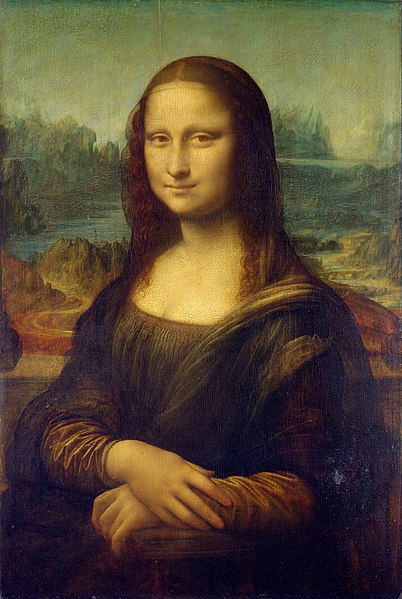
\includegraphics{monalisa}
	\caption[The Mona Lisa]{The Mona Lisa.\\ 
	\url{https://commons.wikimedia.org/wiki/File:Mona_Lisa,_by_Leonardo_da_Vinci,_from_C2RMF_retouched.jpg}}
	\labfig{marginmonalisa}
\end{marginfigure}

The order of the title pages, table of contents and preface can be 
easily changed, as in any \LaTeX\ document. In addition, the class is 
based on \KOMAScript's \Class{scrbook}, therefore it inherits all the 
goodies of that.

\section{What This Class Does Not Do}
\labsec{doesnot}

As anticipated, further customisation of the book is left to the user. 
Indeed, every book may have sidenotes, margin figures and so on, but 
each book will have its own fonts, toc style, special environments and 
so on. For this reason, in addition to the class, we provide only 
sensible defaults, but if these features are not needed, they can be 
left out. These special packages are located in the \Path{style} 
directory, which is organised as follows:

\begin{description}
	\item[kao.sty] This package contains the most important definitions 
	of macros and specifications of page layout. It is the heart of the 
	\Class{kaobook}.
	\item[kaobiblio.sty] Contains commands to add citations and 
	customise the bibliography.
	\item[packages.sty] Loads additional packages to decorate the 
	writing with special contents (for instance, the \Package{listing} 
	package is loaded here as it is not required in every book). There 
	are also defined some useful commands to print the same words always 
	in the same way, \eg latin words in italics or \Package{packages} in 
	verbatim.
	\item[kaorefs.sty] Some useful commands to manage labeling and 
	referencing, again to ensure that the same elements are referenced 
	always in a consistent way.
	\item[environments.sty] Provides special environments, like boxes. 
	Both simple and complex environments are available; by complex we 
	mean that they are endowed with a counter, floating and can be put 
	in a special table of contents.\sidenote[][-2mm]{See 
	\vrefch{mathematics} for some examples.}
	\item[theorems.sty] The style of mathematical environments. 
	Actually, there are two such packages: one is for plain theorems,
	\ie the theorems are printed in plain text; the other uses 
	\Package{mdframed} to draw a box around theorems. You can plug the 
	most appropriate style into its document.
\end{description}

\marginnote[2mm]{The audacious users might feel tempted to edit some of 
these packages. I'd be immensely happy if they sent me examples of what 
they have been able to do!}

In the rest of the book, I shall assume that the reader is not a novice 
in the use of \LaTeX, and refer to the documentation of the packages 
used in this class for things that are already explained there. 
Moreover, I assume that the reader is willing to make minor edits to the 
provided packages for styles, environments and commands, if he or she 
does not like the default settings.

\section{How to Use This Class}

Either if you are using the template from 
\href{http://latextemplates.org/template/kaobook}{latextemplates}, or if 
you cloned the GitHub 
\href{https://www.github.com/fmarotta/kaobook}{repository}, there are 
infinite ways to use the \Class{kaobook} class in practice, but we will 
discuss only two of them. The first is to find the \Path{main.tex} file 
which I used to write this book, and edit it; this will probably involve 
a lot of text-deleting, copying-and-pasting, and rewriting. The second 
way is to start almost from scratch and use the \Path{skeleton.tex} 
file, which is a cleaned-up version of the \Path{main.tex}; even if you 
choose the second way, you may find it useful to draw inspiration from 
the \Path{main.tex} file.

To compile the document, assuming that its name is \Path{main.tex}, you 
will have to run the following sequence of commands:

\begin{lstlisting}[style=kaolstplain,linewidth=1.5\textwidth]
pdflatex main # Compile template
makeindex main.nlo -s nomencl.ist -o main.nls # Compile nomenclature
makeindex main # Compile index
biber main # Compile bibliography
makeglossaries main # Compile glossary
pdflatex main # Compile template again
pdflatex main # Compile template again
\end{lstlisting}

You may need to compile the template some more times in order for some 
errors to disappear. For any support requests, please ask a question on 
\url{tex.stackexchange.org} with the tag \enquote{kaobook}, open an 
issue on GitHub, or contact the author via e-mail.
 % Include the introduction chapter
\chapter{A Chapter of Examples}
\label{chapter1}

\section{A Table}

\begin{table}[h]
\centering
\begin{tabular}{rcc}
\toprule \emph{Feature} & \textsc{Misuse-based} &
\textsc{Anomaly-based}\\
    
\midrule Modeled activity: & Malicious & Normal\\
Detection method: & Matching & Deviation\\
Threats detected: & Known & Any\\
False negatives: & High & Low\\
False positives: & Low & High\\
Maintenance cost: & High & Low\\
Attack desc.: & Accurate & Absent\\
System design: & Easy & Difficult\\
\bottomrule
\end{tabular}
\caption[Duality between misuse- and anomaly-based intrusion detection techniques.]{Duality between misuse- and anomaly-based intrusion detection techniques. Note that, an anomaly-based \ac{IDS} can detect ``Any'' threat, under the assumption that an attack always generates a deviation in the modeled activity.}
\label{tab:misuse-vs-anomaly}
\end{table}

%------------------------------------------------

\section{Code}

\begin{pseudoc}
  /* ... */ cd['<'] = {0.1, 0.11} cd['a'] = {0.01, 0.2} cd['b'] =
  {0.13, 0.23} /* ... */

  b = decode(arg3_value);
  
  if ( !(cd['c'][0] < count('c', b) < cd['c'][1]) ||\
       !(cd['<'][0] < count('<', b) < cd['<'][1]) ||\
       ... || ...)  fire_alert("Anomalous content detected!");
  /* ... */
\end{pseudoc}

%------------------------------------------------

\section{A Sideways Table}

\clearpage
\begin{sidewaystable}
\renewcommand{\arraystretch}{1.5} \centering
\begin{tabular}{rcccccc}
\toprule \textsc{Approach} & \textsc{Time} & \textsc{Header} &
\textsc{Payload} & \textsc{Stochastic} & \textsc{Determ.} & \textsc{Clustering}\\
\midrule \citep{phad} & & $\bullet$ & & & & $\bullet$ \\
\citep{kruegel:sac2002:anomaly} & & $\bullet$ & $\bullet$ & $\bullet$ & & \\
\citep{protocolanom} & & $\bullet$ & & $\bullet$ & $\bullet$ & \\
\citep{ramadas} & & & $\bullet$ & & & $\bullet$ \\
\citep{rules-payl} & $\bullet$ & & $\bullet$ & & $\bullet$ & \\
\citep{zanero-savaresi} & & $\bullet$ & $\bullet$ & & & $\bullet$ \\
\citep{wang:raid2004:payl} & & & $\bullet$ & $\bullet$ & & \\
\citep{zanero-pattern} & & $\bullet$ & $\bullet$ & & & $\bullet$ \\
\citep{DBLP:conf/iwia/BolzoniEHZ06} & & $\bullet$ & $\bullet$ & & & $\bullet$ \\
\citep{wang:raid2006:anagram} & & & $\bullet$ & $\bullet$ & & \\
\bottomrule
\end{tabular}
\caption{Taxonomy of the selected state of the art approaches for network-based anomaly detection.}
\label{tab:network-sota-taxonomy}
\end{sidewaystable}
\clearpage

%------------------------------------------------

\section{A Figure}

\begin{figure}[h]
\centering
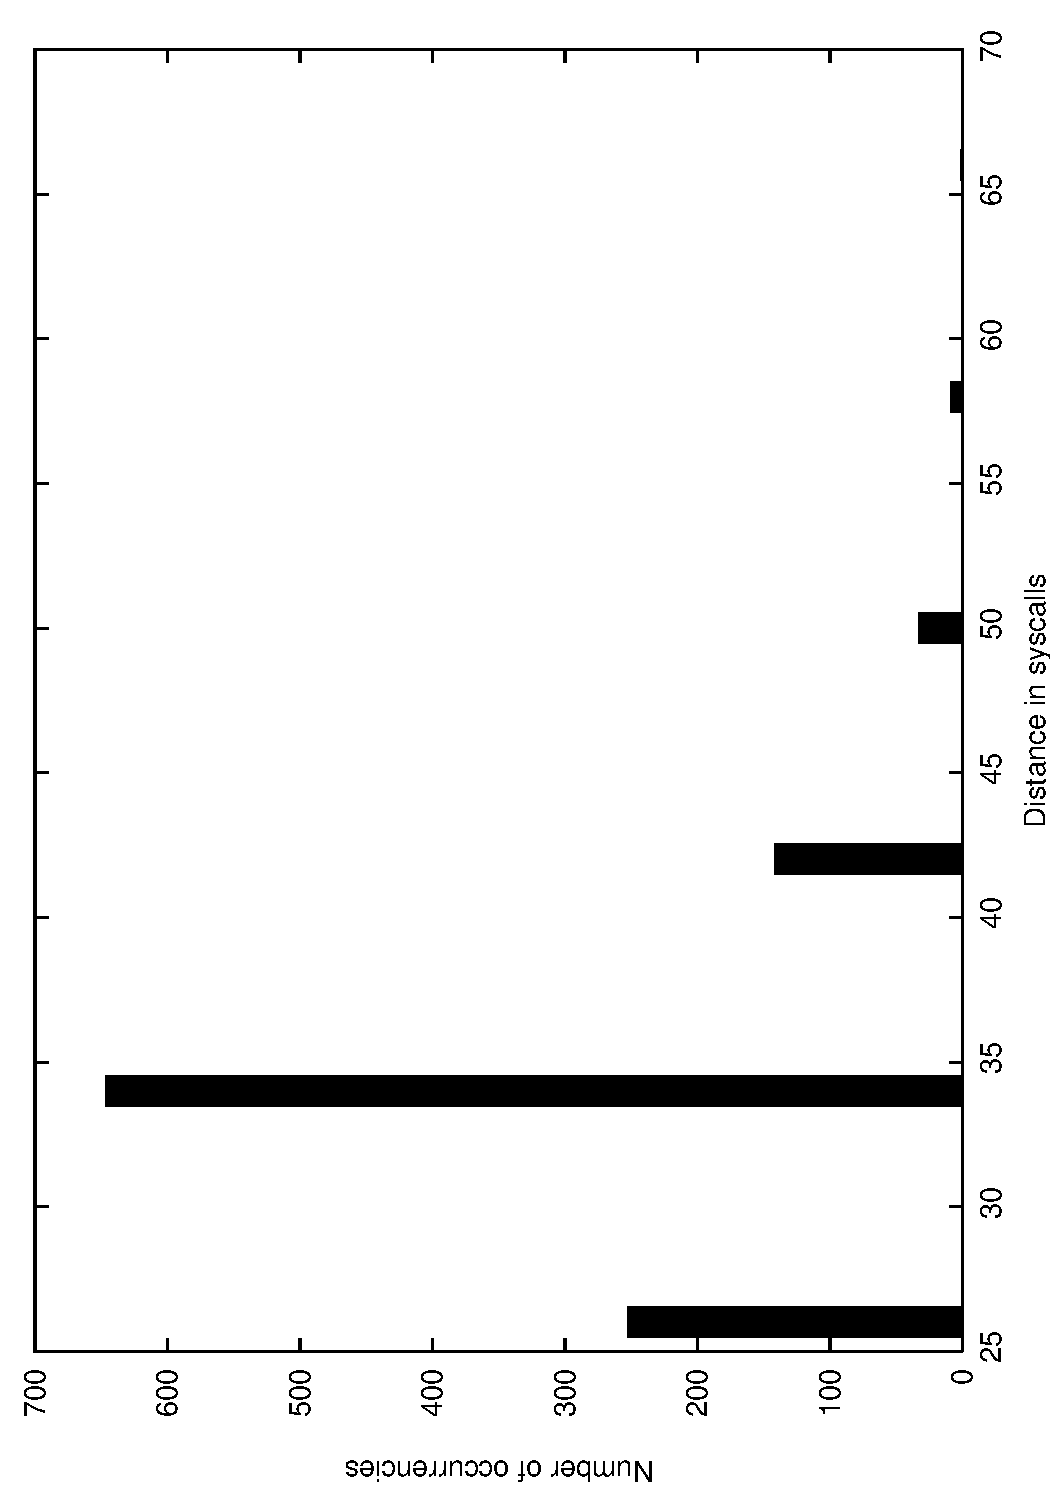
\includegraphics[angle=-90,width=.8\textwidth]{Figures/telnet.pdf}
\caption{\texttt{telnetd}: distribution of the number of other system calls among two \texttt{execve} system calls (i.e., distance between two consecutive \texttt{execve}).}
\label{fig:exectelnet}
\end{figure}

%------------------------------------------------

\section{Bulleted List}

\begin{itemize}
\item $O = $``Intrusion'', $\neg O =$``Non-intrusion'';
\item $A = $``Alert reported'', $\neg A =$``No alert reported''.
\end{itemize}

%------------------------------------------------

\section{Numbered List}

\begin{enumerate}
\item $O = $``Intrusion'', $\neg O =$``Non-intrusion'';
\item $A = $``Alert reported'', $\neg A =$``No alert reported''.
\end{enumerate}

%------------------------------------------------

\section{A Description}

\begin{description}
\item[Time] refers to the use of \emph{timestamp} information, extracted from network packets, to model normal packets. For example, normal packets may be modeled by their minimum and maximum inter-arrival time.
\item[Header] means that the \ac{TCP}\index{TCP} header is decoded and the fields are modeled. For example, normal packets may be modeled by the observed ports range.
\item[Payload] refers to the use of the payload, either at
\ac{IP}\index{IP} or \ac{TCP}\index{TCP} layer. For example, normal packets may be modeled by the most frequent byte in the observed payloads.
\item[Stochastic] means that stochastic techniques are exploited to create models. For example, the model of normal packets may be constructed by estimating the sample mean and variance of certain features (e.g., port number, content length).
\item[Deterministic] means that certain features are modeled following a deterministic approach. For example, normal packets may be only those containing a specified set of values for the \ac{TTL}\index{TTL} field.
\item[Clustering] refers to the use of clustering (and subsequent classification) techniques. For instance, payload byte vectors may be compressed using a \ac{SOM} where class of different packets will stimulate neighbor nodes.
\end{description}

%------------------------------------------------

\section{An Equation}

\begin{equation}
d_a(i,j) := \left\{
\begin{array}{lll}
K_a + \alpha_{a} \delta_{a}(i,j) & \mbox{if the elements are different} \\
0 & \mbox{otherwise}
\end{array}
\right.
\label{eq:distfunction}
\end{equation}

%------------------------------------------------

\section{A Theorem, Proposition \& Proof}

\begin{thm}
$a^2 + b^2 = c^2$
\end{thm}

\begin{prop}
$3 + 3 = 6$
\end{prop}

\begin{proof}
For any finite set $\{p_1,p_2,...,p_n\}$ of primes, consider $m = p_1p_2...p_n+1$. If $m$ is prime it is not in the set since $m > p_i$ for all $i$. If $m$ is not prime it has a prime divisor $p$. If $p$ is one of the $p_i$ then $p$ is a divisor of $p_1p_2...p_n$ and hence is a divisor of $(m - p_1p_2...p_n) = 1$, which is impossible; so $p$ is not in the set. Hence a finite set $\{p_1,p_2,...,p_n\}$ cannot be the collection of all primes.
\end{proof}

%------------------------------------------------

\section{Definition}

\begin{definition}[Anomaly-based \ac{IDS}]
An \emph{anomaly-based \ac{IDS}} is a type of \ac{IDS} that generate alerts $\mathbb{A}$ by relying on normal activity profiles.
\end{definition}

%------------------------------------------------

\section{A Remark}

\begin{rem}
Although the network stack implementation may vary from system to system (e.g., \textsf{Windows} and \textsf{Cisco} platforms have different implementation of \ac{TCP}).
\end{rem}

%------------------------------------------------

\section{An Example}

\begin{example}[Misuse \emph{vs.} Anomaly]\label{ex:misuse-vs-anomaly}
A misuse-based system $M$ and an anomaly-based system $A$ process the same log containing a full dump of the system calls invoked by the kernel of an audited machine. Log entries are in the form:

\begin{center}\small
\begin{verbatim} <function_name>(<arg1_value>, <arg2_value>, ...)
\end{verbatim}
\end{center}
\end{example}

%------------------------------------------------

\section{Note}

\begin{note}[Inspection layer]\label{note:network-stack-standardized}
Although the network stack implementation may vary from system to system (e.g., \textsf{Windows} and \textsf{Cisco} platforms have different implementation of \ac{TCP}), it is important to underline that the notion of IP, TCP, HTTP \emph{packet} is well defined in a system-agnostic way, while the notion of \emph{operating system activity} is rather vague and by no means standardized.
\end{note}
 % Include the first content chapter
%%!TEX root = ../thesis.tex
%*******************************************************************************
%****************************** Second Chapter *********************************
%*******************************************************************************

\chapter{My second chapter}

\ifpdf
    \graphicspath{{Chapter2/Figs/Raster/}{Chapter2/Figs/PDF/}{Chapter2/Figs/}}
\else
    \graphicspath{{Chapter2/Figs/Vector/}{Chapter2/Figs/}}
\fi


\section[Short title]{Reasonably long section title}

% Uncomment this line, when you have siunitx package loaded.
%The SI Units for dynamic viscosity is \si{\newton\second\per\metre\squared}.
I'm going to randomly include a picture Figure~\ref{fig:minion}.


If you have trouble viewing this document contact Krishna at: \href{mailto:kks32@cam.ac.uk}{kks32@cam.ac.uk} or raise an issue at \url{https://github.com/kks32/phd-thesis-template/}


\begin{figure}[htbp!] 
\centering    

\includegraphics[width=1.0\textwidth]{minion}
\caption[Minion]{This is just a long figure caption for the minion in Despicable Me from Pixar}
\label{fig:minion}
\end{figure}


\section*{Enumeration}
Lorem ipsum dolor sit amet, consectetur adipiscing elit. Sed vitae laoreet lectus. Donec lacus quam, malesuada ut erat vel, consectetur eleifend tellus. Aliquam non feugiat lacus. Interdum et malesuada fames ac ante ipsum primis in faucibus. Quisque a dolor sit amet dui malesuada malesuada id ac metus. Phasellus posuere egestas mauris, sed porta arcu vulputate ut. Donec arcu erat, ultrices et nisl ut, ultricies facilisis urna. Quisque iaculis, lorem non maximus pretium, dui eros auctor quam, sed sodales libero felis vel orci. Aliquam neque nunc, elementum id accumsan eu, varius eu enim. Aliquam blandit ante et ligula tempor pharetra. Donec molestie porttitor commodo. Integer rutrum turpis ac erat tristique cursus. Sed venenatis urna vel tempus venenatis. Nam eu rhoncus eros, et condimentum elit. Quisque risus turpis, aliquam eget euismod id, gravida in odio. Nunc elementum nibh risus, ut faucibus mauris molestie eu.
 Vivamus quis nunc nec nisl vulputate fringilla. Duis tempus libero ac justo laoreet tincidunt. Fusce sagittis gravida magna, pharetra venenatis mauris semper at. Nullam eleifend felis a elementum sagittis. In vel turpis eu metus euismod tempus eget sit amet tortor. Donec eu rhoncus libero, quis iaculis lectus. Aliquam erat volutpat. Proin id ullamcorper tortor. Fusce vestibulum a enim non volutpat. Nam ut interdum nulla. Proin lacinia felis malesuada arcu aliquet fringilla. Aliquam condimentum, tellus eget maximus porttitor, quam sem luctus massa, eu fermentum arcu diam ac massa. Praesent ut quam id leo molestie rhoncus. Praesent nec odio eget turpis bibendum eleifend non sit amet mi. Curabitur placerat finibus velit, eu ultricies risus imperdiet ut. Suspendisse lorem orci, luctus porta eros a, commodo maximus nisi.

Nunc et dolor diam. Phasellus eu justo vitae diam vehicula tristique. Vestibulum vulputate cursus turpis nec commodo. Etiam elementum sit amet erat et pellentesque. In eu augue sed tortor mollis tincidunt. Mauris eros dui, sagittis vestibulum vestibulum vitae, molestie a velit. Donec non felis ut velit aliquam convallis sit amet sit amet velit. Aliquam vulputate, elit in lacinia lacinia, odio lacus consectetur quam, sit amet facilisis mi justo id magna. Curabitur aliquet pulvinar eros. Cras metus enim, tristique ut magna a, interdum egestas nibh. Aenean lorem odio, varius a sollicitudin non, cursus a odio. Vestibulum ante ipsum primis in faucibus orci luctus et ultrices posuere cubilia Curae; 
\begin{enumerate}
\item The first topic is dull
\item The second topic is duller
\begin{enumerate}
\item The first subtopic is silly
\item The second subtopic is stupid
\end{enumerate}
\item The third topic is the dullest
\end{enumerate}
Morbi bibendum est aliquam, hendrerit dolor ac, pretium sem. Nunc molestie, dui in euismod finibus, nunc enim viverra enim, eu mattis mi metus id libero. Cras sed accumsan justo, ut volutpat ipsum. Nam faucibus auctor molestie. Morbi sit amet eros a justo pretium aliquet. Maecenas tempor risus sit amet tincidunt tincidunt. Curabitur dapibus gravida gravida. Vivamus porta ullamcorper nisi eu molestie. Ut pretium nisl eu facilisis tempor. Nulla rutrum tincidunt justo, id placerat lacus laoreet et. Sed cursus lobortis vehicula. Donec sed tortor et est cursus pellentesque sit amet sed velit. Proin efficitur posuere felis, porta auctor nunc. Etiam non porta risus. Pellentesque lacinia eros at ante iaculis, sed aliquet ipsum volutpat. Suspendisse potenti.

Ut ultrices lectus sed sagittis varius. Nulla facilisi. Nullam tortor sem, placerat nec condimentum eu, tristique eget ex. Nullam pretium tellus ut nibh accumsan elementum. Aliquam posuere gravida tellus, id imperdiet nulla rutrum imperdiet. Nulla pretium ullamcorper quam, non iaculis orci consectetur eget. Curabitur non laoreet nisl. Maecenas lacinia, lorem vel tincidunt cursus, odio lorem aliquet est, gravida auctor arcu urna id enim. Morbi accumsan bibendum ipsum, ut maximus dui placerat vitae. Nullam pretium ac tortor nec venenatis. Nunc non aliquet neque. 

\section*{Itemize}
\begin{itemize}
\item The first topic is dull
\item The second topic is duller
\begin{itemize}
\item The first subtopic is silly
\item The second subtopic is stupid
\end{itemize}
\item The third topic is the dullest
\end{itemize}

\section*{Description}
\begin{description}
\item[The first topic] is dull
\item[The second topic] is duller
\begin{description}
\item[The first subtopic] is silly
\item[The second subtopic] is stupid
\end{description}
\item[The third topic] is the dullest
\end{description}


\clearpage

\tochide\section{Hidden section}
\textbf{Lorem ipsum dolor sit amet}, \textit{consectetur adipiscing elit}. In magna nisi, aliquam id blandit id, congue ac est. Fusce porta consequat leo. Proin feugiat at felis vel consectetur. Ut tempus ipsum sit amet congue posuere. Nulla varius rutrum quam. Donec sed purus luctus, faucibus velit id, ultrices sapien. Cras diam purus, tincidunt eget tristique ut, egestas quis nulla. Curabitur vel iaculis lectus. Nunc nulla urna, ultrices et eleifend in, accumsan ut erat. In ut ante leo. Aenean a lacinia nisl, sit amet ullamcorper dolor. Maecenas blandit, tortor ut scelerisque congue, velit diam volutpat metus, sed vestibulum eros justo ut nulla. Etiam nec ipsum non enim luctus porta in in massa. Cras arcu urna, malesuada ut tellus ut, pellentesque mollis risus.Morbi vel tortor imperdiet arcu auctor mattis sit amet eu nisi. Nulla gravida urna vel nisl egestas varius. Aliquam posuere ante quis malesuada dignissim. Mauris ultrices tristique eros, a dignissim nisl iaculis nec. Praesent dapibus tincidunt mauris nec tempor. Curabitur et consequat nisi. Quisque viverra egestas risus, ut sodales enim blandit at. Mauris quis odio nulla. Cras euismod turpis magna, in facilisis diam congue non. Mauris faucibus nisl a orci dictum, et tempus mi cursus.

Etiam elementum tristique lacus, sit amet eleifend nibh eleifend sed \footnote{My footnote goes blah blah blah! \dots}. Maecenas dapibu augue ut urna malesuada, non tempor nibh mollis. Donec sed sem sollicitudin, convallis velit aliquam, tincidunt diam. In eu venenatis lorem. Aliquam non augue porttitor tellus faucibus porta et nec ante. Proin sodales, libero vitae commodo sodales, dolor nisi cursus magna, non tincidunt ipsum nibh eget purus. Nam rutrum tincidunt arcu, tincidunt vulputate mi sagittis id. Proin et nisi nec orci tincidunt auctor et porta elit. Praesent eu dolor ac magna cursus euismod. Integer non dictum nunc.


\begin{landscape}

\section*{Subplots}
I can cite Wall-E (see Fig.~\ref{fig:WallE}) and Minions in despicable me (Fig.~\ref{fig:Minnion}) or I can cite the whole figure as Fig.~\ref{fig:animations}


\begin{figure}
  \centering
  \begin{subfigure}[b]{0.3\textwidth}
    
\includegraphics[width=\textwidth]{TomandJerry}
    \caption{Tom and Jerry}
    \label{fig:TomJerry}   
  \end{subfigure}             
  \begin{subfigure}[b]{0.3\textwidth}
    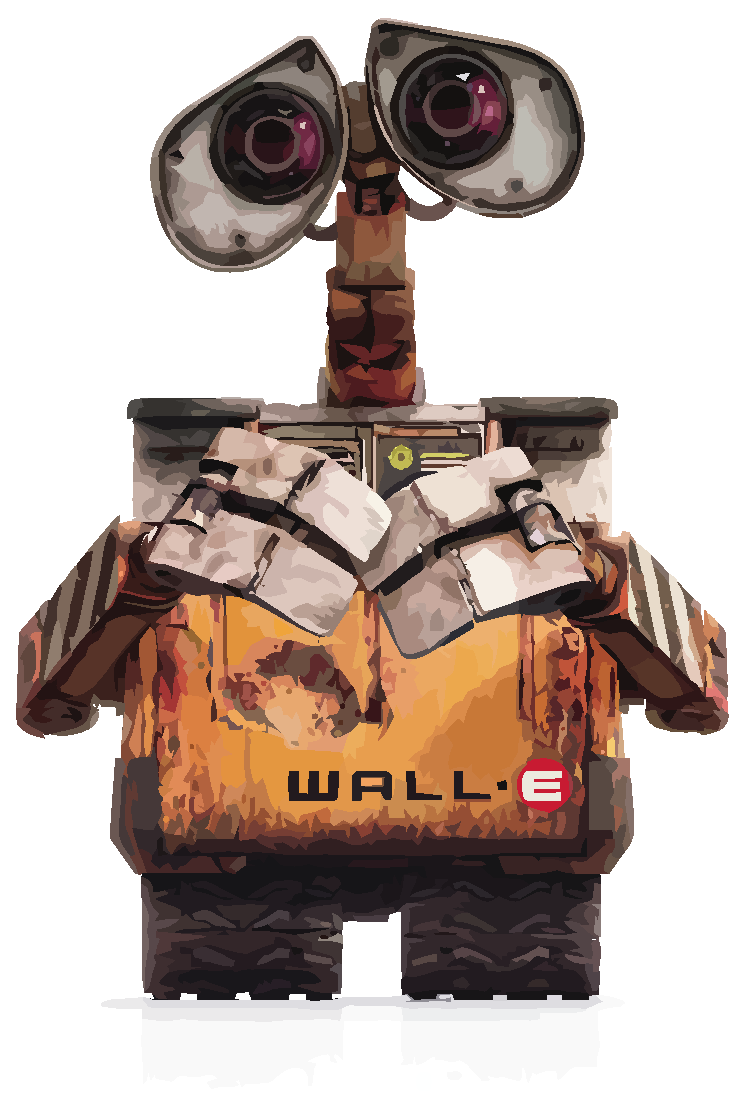
\includegraphics[width=\textwidth]{WallE}
    \caption{Wall-E}
    \label{fig:WallE}
  \end{subfigure}             
  \begin{subfigure}[b]{0.3\textwidth}
    
\includegraphics[width=\textwidth]{minion}
    \caption{Minions}
    \label{fig:Minnion}
  \end{subfigure}
  \caption{Best Animations}
  \label{fig:animations}
\end{figure}


\end{landscape}
 % Include the second content chapter
%%!TEX root = ../thesis.tex
%*******************************************************************************
%****************************** Third Chapter **********************************
%*******************************************************************************
\chapter{My third chapter}

% **************************** Define Graphics Path **************************
\ifpdf
    \graphicspath{{Chapter3/Figs/Raster/}{Chapter3/Figs/PDF/}{Chapter3/Figs/}}
\else
    \graphicspath{{Chapter3/Figs/Vector/}{Chapter3/Figs/}}
\fi

\section{First section of the third chapter}
And now I begin my third chapter here \dots

And now to cite some more people~\citet{Rea85,Ancey1996}

\subsection{First subsection in the first section}
\dots and some more 

\subsection{Second subsection in the first section}
\dots and some more \dots

\subsubsection{First subsub section in the second subsection}
\dots and some more in the first subsub section otherwise it all looks the same
doesn't it? well we can add some text to it \dots

\subsection{Third subsection in the first section}
\dots and some more \dots

\subsubsection{First subsub section in the third subsection}
\dots and some more in the first subsub section otherwise it all looks the same
doesn't it? well we can add some text to it and some more and some more and
some more and some more and some more and some more and some more \dots

\subsubsection{Second subsub section in the third subsection}
\dots and some more in the first subsub section otherwise it all looks the same
doesn't it? well we can add some text to it \dots

\section{Second section of the third chapter}
and here I write more \dots

\section{The layout of formal tables}
This section has been modified from ``Publication quality tables in \LaTeX*''
 by Simon Fear.

The layout of a table has been established over centuries of experience and 
should only be altered in extraordinary circumstances. 

When formatting a table, remember two simple guidelines at all times:

\begin{enumerate}
  \item Never, ever use vertical rules (lines).
  \item Never use double rules.
\end{enumerate}

These guidelines may seem extreme but I have
never found a good argument in favour of breaking them. For
example, if you feel that the information in the left half of
a table is so different from that on the right that it needs
to be separated by a vertical line, then you should use two
tables instead. Not everyone follows the second guideline:

There are three further guidelines worth mentioning here as they
are generally not known outside the circle of professional
typesetters and subeditors:

\begin{enumerate}\setcounter{enumi}{2}
  \item Put the units in the column heading (not in the body of
          the table).
  \item Always precede a decimal point by a digit; thus 0.1
      {\em not} just .1.
  \item Do not use `ditto' signs or any other such convention to
      repeat a previous value. In many circumstances a blank
      will serve just as well. If it won't, then repeat the value.
\end{enumerate}

A frequently seen mistake is to use `\textbackslash begin\{center\}' \dots `\textbackslash end\{center\}' inside a figure or table environment. This center environment can cause additional vertical space. If you want to avoid that just use `\textbackslash centering'


\begin{table}
\caption{A badly formatted table}
\centering
\label{table:bad_table}
\begin{tabular}{|l|c|c|c|c|}
\hline 
& \multicolumn{2}{c}{Species I} & \multicolumn{2}{c|}{Species II} \\ 
\hline
Dental measurement  & mean & SD  & mean & SD  \\ \hline 
\hline
I1MD & 6.23 & 0.91 & 5.2  & 0.7  \\
\hline 
I1LL & 7.48 & 0.56 & 8.7  & 0.71 \\
\hline 
I2MD & 3.99 & 0.63 & 4.22 & 0.54 \\
\hline 
I2LL & 6.81 & 0.02 & 6.66 & 0.01 \\
\hline 
CMD & 13.47 & 0.09 & 10.55 & 0.05 \\
\hline 
CBL & 11.88 & 0.05 & 13.11 & 0.04\\ 
\hline 
\end{tabular}
\end{table}

\begin{table}
\caption{A nice looking table}
\centering
\label{table:nice_table}
\begin{tabular}{l c c c c}
\hline 
\multirow{2}{*}{Dental measurement} & \multicolumn{2}{c}{Species I} & \multicolumn{2}{c}{Species II} \\ 
\cline{2-5}
  & mean & SD  & mean & SD  \\ 
\hline
I1MD & 6.23 & 0.91 & 5.2  & 0.7  \\

I1LL & 7.48 & 0.56 & 8.7  & 0.71 \\

I2MD & 3.99 & 0.63 & 4.22 & 0.54 \\

I2LL & 6.81 & 0.02 & 6.66 & 0.01 \\

CMD & 13.47 & 0.09 & 10.55 & 0.05 \\

CBL & 11.88 & 0.05 & 13.11 & 0.04\\ 
\hline 
\end{tabular}
\end{table}


\begin{table}
\caption{Even better looking table using booktabs}
\centering
\label{table:good_table}
\begin{tabular}{l c c c c}
\toprule
\multirow{2}{*}{Dental measurement} & \multicolumn{2}{c}{Species I} & \multicolumn{2}{c}{Species II} \\ 
\cmidrule{2-5}
  & mean & SD  & mean & SD  \\ 
\midrule
I1MD & 6.23 & 0.91 & 5.2  & 0.7  \\

I1LL & 7.48 & 0.56 & 8.7  & 0.71 \\

I2MD & 3.99 & 0.63 & 4.22 & 0.54 \\

I2LL & 6.81 & 0.02 & 6.66 & 0.01 \\

CMD & 13.47 & 0.09 & 10.55 & 0.05 \\

CBL & 11.88 & 0.05 & 13.11 & 0.04\\ 
\bottomrule
\end{tabular}
\end{table}
 % Include the third content chapter

\backmatter

\chapterstyle{default} % Reset the chapter style back to the default used for non-content chapters

%----------------------------------------------------------------------------------------
%	BIBLIOGRAPHY
%----------------------------------------------------------------------------------------

\bibliographystyle{plainnat} % Use the plainnat bibliography style

\bibliography{bibliography} % Use the bibliography.bib file as the source of references

%----------------------------------------------------------------------------------------
%	INDEX
%----------------------------------------------------------------------------------------

\printindex % Print the index

%----------------------------------------------------------------------------------------

\end{document}